% Nama Kelompok : Kelompok 2
% Kelas : D4 TI 1A
% 1. Kadek Diva Krishna Murti (1174006)
% 2. Duvan Silalahi (1174011)
% 3. Oniwaldus (1174005)
% 4. Choirul Anam (1174004)
% 5. Sri Rahayu (1174015)
% 6. Ilham Habibi (1174028)

%\documentclass{article}

%\usepackage{amsmath}
%\usepackage{textcomp}
%\usepackage{graphicx}
%\usepackage{enumitem}
%\usepackage{verbatim}

%\begin{document}

\section{Pengertian} 

\begin{figure}[ht]
\centerline{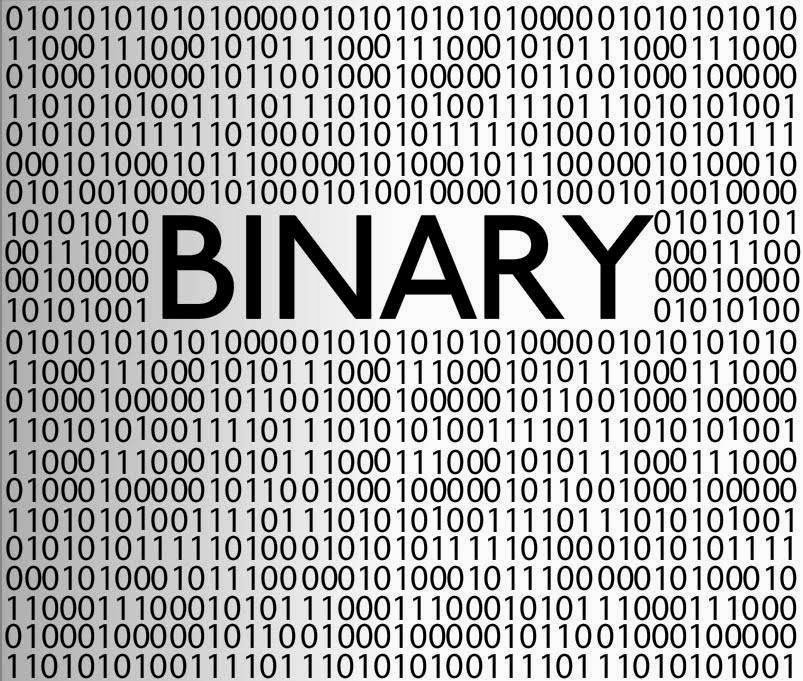
\includegraphics[width=0.4\textwidth]{figures/biner.jpg}}
\caption{Sistem bilangan biner.}
\label{biner}
\end{figure}

Sejak Personal Computer (PC) atau komputer pertama kali ditemukan, komputer tersebut telah beroperasi menggunakan sistem bilangan biner. Bilangan biner merupakan bilangan yang berbasis dua pada sistem bilangan. Semua data dan kode program pada komputer dimanipulasi serta disimpan dalam format biner yang merupakan kode - kode mesin komputer. Sehingga semua perhitungan – perhitungan yang diolah oleh computer tersebut menggunakan aritmatika biner yang hasilnya berupa bilangan hanya memiliki dua kemungkinan nilai, yaitu 0 dan 1. 

\begin{figure}[ht]
\centerline{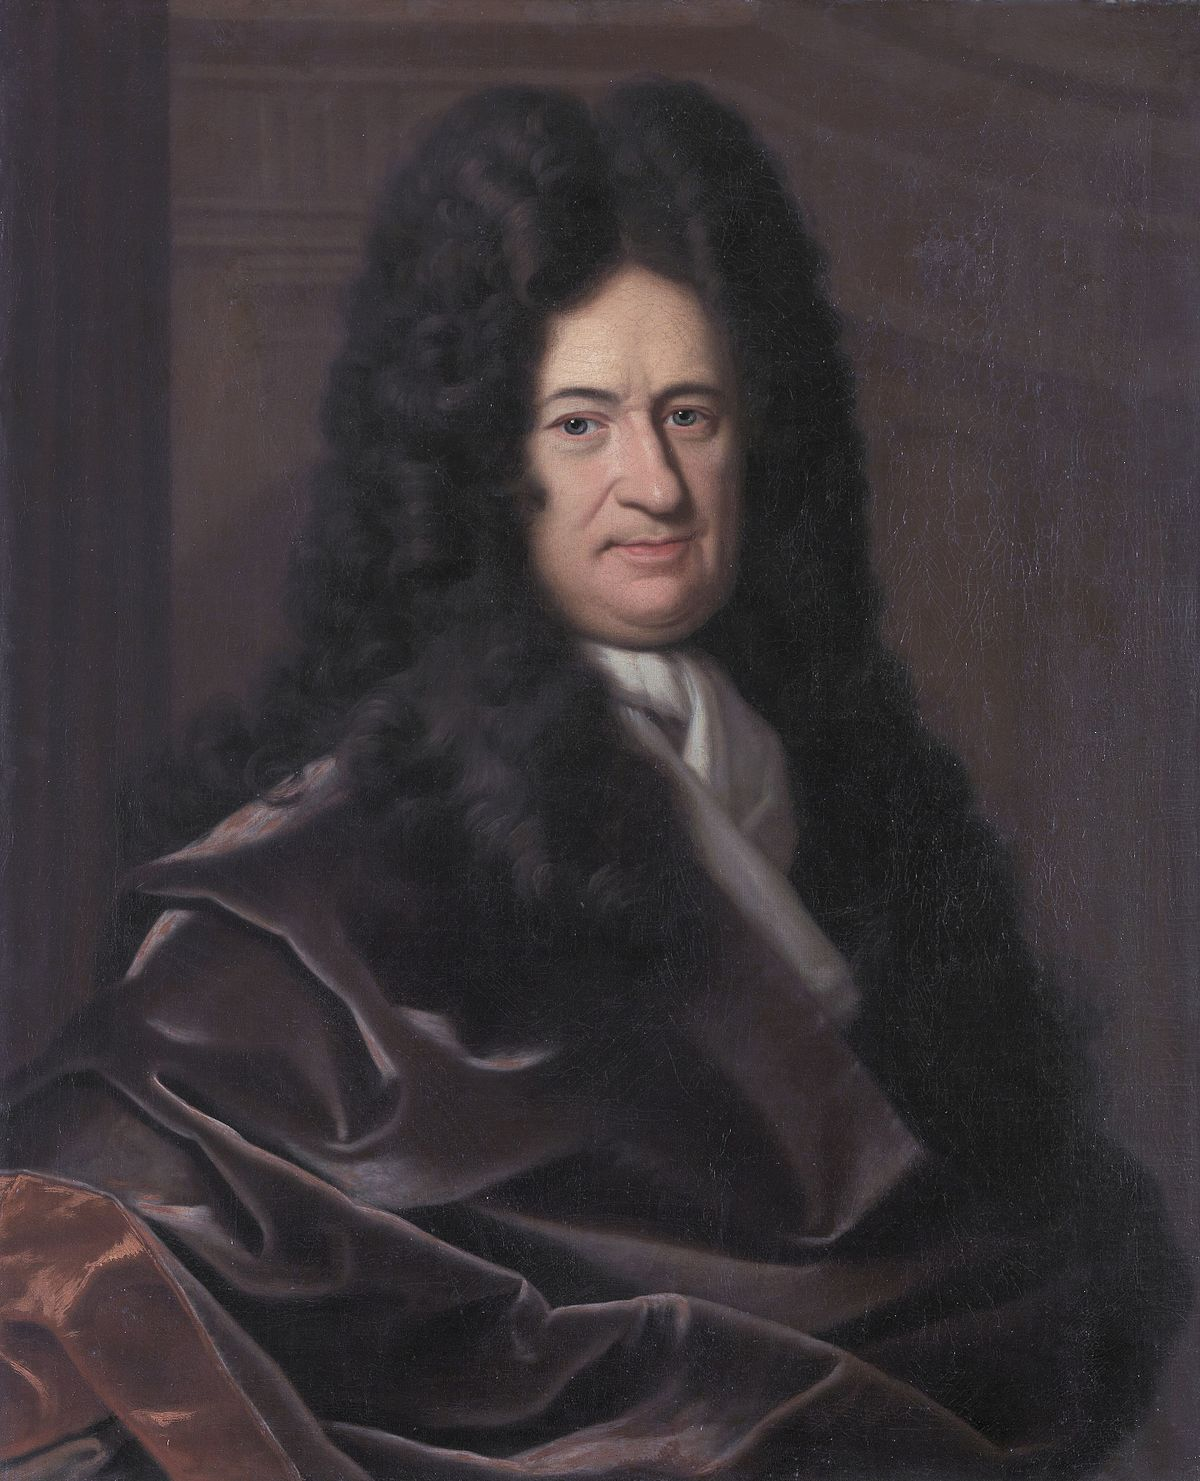
\includegraphics[width=0.4\textwidth]{figures/gwl.jpg}}
\caption{Penemu sistem bilangan biner.}
\label{gwl}
\end{figure}

Dikutip dari \cite{hutahaean2015konsep} bilangan biner \ref{biner} atau bilangan berbasis dua atau binary dalam Bahasa Inggris merupakan sebuah penulisan bilangan di mana bilangan – bilangan tersebut hanya menggunakan dua angka, yaitu 0 dan 1. Tidak seperti bilangan desimal yang merupakan sistem bilangan berbasis 10, sistem bilangan biner berbasis 2. bilangan biner digunakan untuk informasi biner dan juga satuan ukuran besarnya data. Sistem bilangan biner modern ditemukan oleh Gottfried Wilhelm Leibniz \ref{gwl} pada abad ke-17. Sistem bilangan ini merupakan dasar dari semua sistem bilangan berbasis digital. Dari sistem biner tersebut, kita dapat mengkonversinya ke sistem bilangan Hexadesimal atau Oktal. Sistem ini juga dapat kita sebut dengan istilah bit atau Binary Digit atau dalam arsitektur elektronik biasa disebut sebagai digital logic.. 

Pengelompokan biner dalam sebuah Personal Computer atau komputer selalu memilki jumlah 8, dengan istilah 1 Byte atau bita. Dalam istilah komputer 1 Byte = 8 bit. Kode-kode rancang bangun komputer seperti American Standard Code for Information Interchange (ASCII) menggunakan sistem pengkodean 1 Byte. Bilangan biner digunakan untuk satuan ukuran besarnya data dan juga informasi biner.

 
Pada bilangan biner setiap digitnya mewakili pangkat pada angka 2 yang terus meningkat dari kanan ke kiri, Digit yang paling kanan mewakili 2 pangkat 0 ($2^0$). Digit selanjutnya mewakili 2 pangkat 1 ($2^1$), selanjutnya lagi mewakili 2 pangkat 2 ($2^2$), begitu juga seterusnya. Pada bilangan biner, angka 0 pada bilangan desimal diwakili dengan bilangan biner '0', begitu juga dengan angka 1 pada bilangan desimal diwakili dengan bilangan biner '1'. Kedua bilangan 0 dan 1 tersebut tidak berubah. Bilangan desimal 2 diwakili sebagai bilangan biner '10', 3 sebagai '11', 4 sebagai '100', 5 sebagai '101', begitu juga seterusnya.

Dalam sistem komunikasi digital modern, dimana data ditransmisikan dalam bentuk bit-bit biner, dibutuhkan sistem yang tahan terhadap noise yang terdapat di kanal transmisi sehingga data yang ditransmisikan tersebut dapat diterima dengan benar. Kesalahan dalam suatu penerimaan atau pengiriman data merupakan permasalahan yang paling mendasar dan memberikan dampak yang sangat signifikan pada sistem komunikasi. Biner yang biasa dipakai itu ada 8 digit angka dan cuma berisikan angka 1 dan 0, tidak ada angka lainnya.

Posisi sebuah angka dalam bilangn biner atau bilangan basis dua akan menentukan berapa bobot nilainya. Posisi paling depan (kiri) sebuah bilangan memiliki nilai yang paling besar sehingga disebut sebagai MSB (Most Significant Bit), dan posisi paling belakang (kanan) sebuah bilangan memiliki nilai yang paling kecil sehingga disebut sebagai LSB (Leased Significant Bit). Berikut ini adalah contoh representasi dari bilangan biner atau bilangan berbasis dua : 
$10110_2$ = 1 x $2^4$ + 0 x $2^3$ + 1 x $2^2$ + 1 x $2^1$ + 0 x $2^0$ = $22_{10}$

\subsection{Bilangan Biner}
\qquad Sebagai perumpamaan untuk bilangan desimal, untuk angka 157 : $157_{(10)}$ = (1 x 100) + (5 x 10) + (7 x 1) \\

Perhatikan! Bilangan desimal atau sering juga disebut dengan basis 10. Hal ini dikarenakan perpangkatan 10 yang didapat dari 100, 101, 102, dst. 

\subsubsection{Mengenal Konsep Bilangan Biner dan Desimal}
\qquad Perbedaan paling mendasar dari metode bilangan biner dan bilangan desimal terletak pada jumlah dari basisnya. Jika desimal berbasis 10 (x10) berpangkatkan 10x, maka untuk bilangan biner berbasiskan 2 (x2) menggunakan perpangkatan 2x.
Sederhananya perhatikan contoh dibawah ini!\\
Untuk Desimal:
\begin{table}[h!]
\begin{tabular}{ l l }
$14_{(10)}$ & = (1 x $10^1$) + (4 x $10^0$)\\
& = 10 + 4\\
& = 14\\
\end{tabular}
\end{table}
\\
Untuk Biner:
\begin{table}[h!]
\begin{tabular}{ l l }
$1110_{(2)}$ & = (1 x $2^3$) + (1 x $2^2$) + (1 x $2^1$) + (0 x $2^0$)\\
& = 8 + 4 + 2 + 0\\
& = 14\\
\end{tabular}
\end{table}

Bentuk umum dari bilangan biner dan bilangan desimal bisa dilihat pada tabel \ref{table:binerdesimal}. 

\begin{table}[h!]
\centering
\begin{tabular}{ |c|c|c|c|c|c|c|c|c|c| } 
\hline
Biner & 1 & 1 & 1 & 1 & 1 & 1 & 1 & 1 & 11111111 \\ 
\hline
Desimal & 128 & 64 & 32 & 16 & 8 & 4 & 2 & 1 & 255 \\ 
\hline
Pangkat & $2^7$ & $2^6$ & $2^5$ & $2^4$ & $2^3$ & $2^2$ & $2^1$ & $2^0$ & $X^{1-7}$ \\ 
\hline
\end{tabular}
\caption{Tabel bentuk umum dari bilangan biner dan bilangan desimal}
\label{table:binerdesimal}
\end{table}

Sekarang kita kembali lagi ke contoh soal di atas! Darimana kita dapatkan angka desimal 14(10) menjadi angka biner 1110(2)? 
Mari kita lihat lagi pada bentuk umumnya pada tabel \ref{table:contoh1}!

\begin{table}[h!]
\centering
\begin{tabular}{ |c|c|c|c|c|c|c|c|c|c| } 
\hline
Biner & 0 & 0 & 0 & 0 & 1 & 1 & 1 & 0 & 00001110 \\ 
\hline
Desimal & 0 & 0 & 0 & 0 & 8 & 4 & 2 & 0 & 14 \\ 
\hline
Pangkat & $2^7$ & $2^6$ & $2^5$ & $2^4$ & $2^3$ & $2^2$ & $2^1$ & $2^0$ & $X^{1-7}$ \\ 
\hline
\end{tabular}
\caption{Tabel contoh biner ke desimal.}
\label{table:contoh1}
\end{table}

\noindent Mari kita telusuri perlahan-lahan!

\begin{enumerate}[label=(\alph*)]
\item Pertama, kita jumlahkan angka pada desimal sehingga menjadi 14. Pada tabel lihat angka – angka mana yang menghasilkan angka 14 adalah 8, 4, dan juga 2!
\item Untuk angka-angka yang membentuk angka 14 (lihat angka yang diarsir), diberi tanda biner "1", selebihnya diberi tanda "0".
\item Jadi apabila dibaca dari kanan, angka desimal 14 akan menjadi 00001110 (terkadang dibaca 1110) pada angka binernya.
\end{enumerate}


\subsubsection{Mengubah Angka Biner ke Desimal}
Perhatikan contoh! 

\begin{enumerate}[label=(\alph*)]
\item $11001101_{(2)}$ 

\begin{table}[h!]
\centering
\begin{tabular}{ |c|c|c|c|c|c|c|c|c|c| } 
\hline
Biner & 1 & 1 & 0 & 0 & 1 & 1 & 0 & 1 & 11001101 \\ 
\hline
Desimal & 128 & 64 & 0 & 0 & 8 & 4 & 0 & 1 & 205 \\ 
\hline
Pangkat & $2^7$ & $2^6$ & $2^5$ & $2^4$ & $2^3$ & $2^2$ & $2^1$ & $2^0$ & $X^{1-7}$ \\ 
%%%%%%%%%%%%%
\hline
\end{tabular}
\caption{Tabel contoh biner ke desimal.}
\label{table:contoh2}
\end{table}

Note:
\begin{itemize}
\item Pada tabel angka desimal 205 didapat dari penjumlahan angka yang di arsir (128 + 64 + 8 + 4 + 1)
\item Setiap biner yang bertanda "1" akan dihitung, sementara biner yang bertanda "0" tidak dihitung, alias "0" juga.
\end{itemize}

\item $00111100_{(2)}$ 

\begin{table}[h!]
\centering
\begin{tabular}{ |c|c|c|c|c|c|c|c|c|c| } 
\hline
Biner & 0 & 0 & 1 & 1 & 1 & 1 & 0 & 0 & 00111100 \\ 
\hline
Desimal & 0 & 0 & 32 & 16 & 8 & 4 & 0 & 0 & 60 \\ 
\hline
Pangkat & $2^7$ & $2^6$ & $2^5$ & $2^4$ & $2^3$ & $2^2$ & $2^1$ & $2^0$ & $X^{1-7}$ \\ 
\hline
\end{tabular}
\caption{Tabel contoh biner ke desimal.}
\label{table:contoh2}
\end{table}

Note:
\begin{itemize}
\item Pada tabel angka desimal 60 didapat dari penjumlahan angka yang di arsir (32 + 16 + 8 + 4)
\item Setiap biner yang bertanda "1" akan dihitung, sementara biner yang bertanda "0" tidak dihitung, alias "0" juga.
\end{itemize}

\subsubsection {Mengubah Angka Desimal ke Biner} 

\qquad Dalam mengubah angka desimal menjadi angka biner dipergunakan sebuah metode pembagian dengan angka 2 dengan memperhatikan sisanya. 
Perhatikan contohnya! 
\begin{enumerate}
\item $205_{(10)}$\\
205 : 2 = 102 sisa 1\\ 
102 : 2 = 51 sisa 0 \\
51 \,: 2 = 25 sisa 1\\
25 \,: 2 = 12 sisa 1 \\
12 \,: 2 = 6 sisa 0 \\
6 \quad : 2 = 3 sisa 0 \\
3 \quad : 2 = 1 sisa 1 \\
1  sebagai sisa akhir "1"\\

Note :\\
Pembacaan dilakukan dari bawah, untuk menuliskan notasi binernya yang berarti 11001101(2) \\

\item $60_{(10)}$\\
60 : 2 = 30 sisa 0\\ 
30 : 2 = 15 sisa 0 \\
15 : 2 = 7 sisa 1 \\
7  : 2 = 3 sisa 1 \\
3  : 2 = 1 sisa 1 \\
1  sebagai sisa akhir "1"\\

Note :\\
Dibaca dari bawah menjadi 111100(2) atau lazimnya dituliskan dengan 00111100(2). Ingat bentuk umumnnya mengacu untuk 8 digit! Jika 111100 (masih 6 digit) menjadi 00111100 (sudah 8 digit).

\end{enumerate}

\subsection{Aritmatika Biner}

\qquad Pada aritmatika biner akan membahas penjumlahan dan pengurangan biner. Pada bilangan biner perkalian merupakan pengulangan dari penjumlahan bilangan biner dan pengurangan bilangan biner berdasarkan ide atau gagasan komplemen.

\begin{enumerate}

\item Penjumlahan Biner

\qquad Penjumlahan biner tidak begitu beda jauh dengan penjumlahan desimal. Perhatikan contoh penjumlahan desimal antara 167 dan 235.

1 menjadi 7 + 5 = 12, tulis "2" di bawah dan angkat "1" ke atas! \\

167 \\
235 \\
------ + \\
402 \\

\qquad Pada bilangan biner penjumlahan dilakukan dengan cara yang sama seperti pada bilangan desimal. Yang harus dicermati pertama adalah aturan - aturan pasangan digit biner berikut:\\
0 + 0 = 0 \\
0 + 1 = 1 \\
1 + 1 = 0  dan menyimpan 1 \\

sebagai catatan bahwa jumlah dua yang terakhir adalah : \\
1 + 1 + 1 = 1 dan menyimpan 1 \\

\qquad Jadi, hanya dengan menggunakan cara penjumlahan di atas, kita dapat melakukan penjumlahan bilangan biner seperti yang ditunjukkan di bawah ini: \\
1 1111 sebagai "Simpanan 1" ingat kembali aturan di atas! \\
01011011 sebagai Bilangan biner untuk 91 \\
01001110 sebagai Bilangan biner untuk 78 \\
------------ + \\
10101001 sebagai Jumlah dari 91 + 78 = 169 \\

\qquad Kalian juga dapat mempelajari aturan - aturan pasangan digit biner yang telah tertera di atas! Contoh penjumlahan biner yang terdiri dari 5 bilangan!\\
\begin{verbatim}
11101 bilangan 1)
10110 bilangan 2) 
 1100 bilangan 3)
11011 bilangan 4)
 1001 bilangan 5)
----- +
\end{verbatim}

\qquad Untuk menjumlahkan penjumlahan di atas , pertama kita jumlahkan berdasarkan aturan - aturan yang berlaku, dan untuk mempermudah maka perhitungannya dilakukan secara bertahap. \\
\begin{verbatim}
  11101 bilangan 1)
  10110 bilangan 2)
------- +
 110011
   1100 bilangan 3)
------- +
 111111
  11011 bilangan 4)
------- +
 011010
   1001 bilangan 5)
------- +
\end{verbatim}
1100011 sebagai Jumlah Akhir. \\

Berapakah bilangan desimal? \\

Sekarang coba tentukan berapakah bilangan 1,2,3,4 dan 5! Apakah memang perhitungan di atas sudah benar? \\

\item Pengurangan Biner

\qquad Pada pengurangan suatu bilangan desimal 73426 - 9185 akan dihasilkan:
\begin{verbatim}
73426 sebagai Angka 7 dan angka 4 dikurang dengan angka 1
 9185 sebagai Digit desimal pengurang.
----- -
64241 sebagai Hasil dari pengurangan.
\end{verbatim}

Bentuk Umum pengurangan : \\
0 - 0 = 0 \\
1 - 0 = 1 \\
1 - 1 = 0 \\
0 - 1 = 1  dengan meminjam "1" dari digit pada sebelah kirinya! \\
 
\quad Untuk pengurangan pada bilangan biner dapat dilakukan dengan cara yang sama. Coba anda perhatikan bentuk pengurangan berikut ini:
\begin{verbatim}
1111011 sebagai desimal 123
 101001 sebagai desimal 41
--------- -
1010010 sebagai desimal 82 
\end{verbatim}
\qquad Pada contoh di atas tidak terjadi "konsep peminjaman". Perhatikan contoh berikut!

\begin{verbatim}
     0  sebagai kolom ke-3 telah menjadi "0", karena sudah dipinjam!
111101  sebagai desimal 61
 10010  sebagai desimal 18
--------- -
101011  sebagai Hasil pengurangan akhir 43.
\end{verbatim}

\qquad Pada contoh di atas tadi kita meminjam “1” pada kolom 3, karena adanya selisih 0-1 pada kolom ke-2. Lihat Bentuk Umum!
\begin{verbatim}
  7999 sebagai hasil pinjaman
800046
397261
------- -
402705
\end{verbatim}

\qquad Sebagai contoh pengurangan bilangan biner 110001 - 1010 maka diperoleh hasil seperti berikut:
\begin{verbatim}
1100101
   1010
-------- - 
 100111
\end{verbatim}

\item Perkalian Biner

\qquad Perkalian pada bilangan biner pada umumnya sama dengan perkalian pada bilangan desimal, perbedaanya terletak pada nilai yang dihasilkan adalah hanya 0 dan 1. Pada perkalian bilangan biner, bergeser1 ke kanan setiap dikalikan 1 bit pengali. Setelah proses perkalian masing-masing bit pengali sudah selesai, lakukan penjumlahan masing-masing kolom bit hasil.
\begin{verbatim}

%%%%%%%%

   1101 sebagai Yang dikalikan
 x 1011 sebagai Pengali
-----------
   1101
  1101
 0000
1101
---------
1000111
\end{verbatim}


\item Pembagian Biner

\qquad Pembagian pada bilangan biner pada umumnya sama dengan pembagian pada bilangan desimal, perbedaanya terletak pada nilai yang dihasilkan  adalah hanya 0 dan 1. Bit - bit yang dibagi diambil bit per bit dari sebelah kiri. Apabila nilai bilangan biner yang dibagi lebih dari bit bilangan biner pembagi, maka bagilah bit-bit tersebut. Apabila setelah bergeser 1 bit nilainya masih dibawah dari bit pembagi, maka hasil bagi sama dengan 0.
\begin{verbatim}
      11
     -----
011 / 1001 sebagai Yang dibagi
    - 011
    ------
      0011
    - 011
     ------
         0
\end{verbatim}


\item Komplemen

\qquad Metode pengurangan yang digunakn pada komputer biasanya ditransformasikan menjadi penjumlahan dengan mempergunakan komplemen radiks atau minus radiks komplemen satu. Pertama akan dibahas dahulu komplemen pada sistem desimal imana komplemen - komplemen tersebut secara berurutan disebut dengan komplemen sembilan dan komplemen sepuluh (komplemen pada sistem biner disebut dengan komplemen satu dan komplemen dua). Prinsip yang paling penting yang perlu ditanamkan adalah: \\

\qquad "Komplemen sembilan pada bilangan desimal didapat dengan mengurangkan masing - masing digit desimal tersebut ke bilangan 9, sedangkan komplemen sepuluh adalah komplemen sembilan ditambah dengan 1" \\
Lihat contoh nyatanya!\\

\begin{tabular}{ l l l l }
Bilangan Desimal & 123 & 651 & 914 \\
Komplemen Sembilan &876 &348 &085 \\ 
Komplemen Sepuluh &877 &349 &086 sebagai ditambah dengan 1! \\
\end{tabular}\\

\qquad Perhatikan hubungan diantara bilangan dan komplemennya adalah simetris. Maka dari dapat disimpulkan dengan memperhatikan contoh di atas, komplemen 9 dari 123 adalah 876 dengan simpel menjadikan jumlahnya = 9 (1 + 8 = 9, 2 + 7 = 9, 3 + 6 = 9)! \\


\qquad Sementara komplemen 10 didapat dengan cara menambahkan 1 pada komplemen 9, yang berarti 876 + 1 = 877. \\

\qquad Pengurangan desimal dapat dilakukan dengan menggunakan penjumlahan komplemen sembilan plus satu, atau penjumlahan dari komplemen sepuluh. \\


\begin{tabular}{ l l l }
893 &  893 & 893 \\ 
321 &  678 (komp. 9) & 679 (komp. 10) \\
----- - & ----- + & ----- + \\
572 & 1571 & 1572 \\
&  \quad1 & \\
& ----- - & \\
& 572 sebagai angka 1 dihilangkan& \\
\end{tabular}

\end{enumerate}
\qquad Kesimpulan yang dapat diambil dari perhitungan komplemen di atas adalah, komplemen satu dari bilangan biner didapat dengan cara mengurangkan masing - masing digit biner tersebut ke bilangan 1, atau dengan penjelasan singkatnya mengubah masing-masing 0 menjadi 1 atau sebaliknya mengubah masing-masing 1 menjadi 0. Sedangkan komplemen dua merupakan satu plus satu. \\
Perhatikan Contoh. \\

\begin{tabular}{ l l l l }
Bilangan Biner &110011& 101010& 011100 \\
Komplemen Satu& 001100 &010101 &100011 \\
Komplemen Dua& 001101& 010110& 100100 \\
\end{tabular}\\

\quad Contoh pengurangan biner 110001 – 1010 akan dijelaskan pada contoh di bawah ini! \\
110001 \quad110001 \quad110001 \\
001010 \quad110101 \quad110110 \\
----------- - --------- + --------- + \\
100111 \quad100111 \quad1100111 dihilangkan! \\

\qquad Alasan kenapa cara komplemen ini dilakukan, dapat dijelaskan dengan memperhatikan sebuah speedometer mobil atau motor dengan empat digit yang sedang membaca nol. \\

\end{enumerate}

%\end{document}